\documentclass[a4paper,12pt,twopage]{article}

%dit is de preamble voeg hier nieuwe packages toe en declareer nieuwe commando's
\usepackage{amsmath}
\usepackage{graphicx}
\usepackage{color}
\usepackage[english]{babel}
\usepackage{hyperref}
\usepackage{physics}
\usepackage{amssymb}
\usepackage{enumitem}
\usepackage{tikz}
\usetikzlibrary{automata,positioning,calc}
\usepackage{listings}
%\usepackage[version=3]{mhchem}

%zo voeg je een nieuw commando in, als je dat fijn vind. Bestaat het al (LaTeX geeft
%dan een waarschuwing), gebruik dan \renewcommand{}{}. Wees daar wel voorzichtig mee.
\newcommand{\figuurbreedte}{56mm}
\newcommand{\commando}[1]{\texttt{$\backslash$#1}}
\newcommand\tab[1][1cm]{\hspace*{#1}}

%met het onderstaande maak je de marges links rechts boven en onder kleiner
\addtolength{\hoffset}{-1cm}
\addtolength{\textwidth}{2cm}
\addtolength{\voffset}{-1.5cm}
\addtolength{\textheight}{3cm}
\usepackage{float}


\author{Mark Beijer, s4354834}
\date{}
\title{}
\definecolor{mygreen}{rgb}{0,0.6,0}
\definecolor{mygray}{rgb}{0.5,0.5,0.5}
\definecolor{mymauve}{rgb}{0.58,0,0.82}

\lstset{ %
  backgroundcolor=\color{white},   % choose the background color
  basicstyle=\footnotesize,        % size of fonts used for the code
  breaklines=true,                 % automatic line breaking only at whitespace
  captionpos=b,                    % sets the caption-position to bottom
  commentstyle=\color{mygreen},    % comment style
  escapeinside={\%*}{*)},          % if you want to add LaTeX within your code
  keywordstyle=\color{blue},       % keyword style
  stringstyle=\color{mymauve},     % string literal style
}

\begin{document}

\maketitle


\section{Exercise 2}

\begin{enumerate}
\item

I made the function using the following code:


\begin{lstlisting}[language=Python]
def H(x,y):
    return 100*(y-x**2)**2+(1-x)**2
\end{lstlisting}

This returns h as defined by (7) in the assignment.

To create the data I used the following code:

\begin{lstlisting}[language=Python]
Amount = 1000
xmin = -2
xmax = 2
ymin = -1
ymax = 3
x = np.linspace(xmin,xmax,Amount)
y = np.linspace(ymin,ymax,Amount)
x,y = np.meshgrid(x,y)
z = H(x,y)
\end{lstlisting}

This first creates a row of 1000 numbers, with the boundaries as given in the assignment. Then the meshgrid function a 2d array so every combination $(x_i,y_i)$ in these boundaries is found at some (x[i,j],y[i,j]). Then we calculate z using our function.

For plotting I used the following code:

\begin{lstlisting}[language=Python]
fig = plt.figure()
ax = fig.gca(projection='3d')
surf = ax.plot_surface(x, y, z, cmap=cm.coolwarm,
                       linewidth=0, antialiased=False)
fig.colorbar(surf, shrink=0.5, aspect=5)
\end{lstlisting}


This creates a figure and axes to plot on. Then I used a surface plot which takes the 2d x,y,z values and plots them. I used a colormap to also show the value of z using colors. The last line plots this colorbar.

It looks like the function is quite steep and so the numerical minimization with gradient descent might be fast. For if it's steep it will make a big jump towards the minimum with the gradient descent rule.


\item

The gradient of h is given by:

\begin{equation}
\nabla h(x,y) = \begin{bmatrix}
200(y-x^2)\cdot -2x -(1-x)\cdot 2\\
200(y-x^2)
\end{bmatrix} = \begin{bmatrix}
400x^3-400xy+2x-2\\
200y-200x^2
\end{bmatrix}
\end{equation}

Now if we fill in the point (1,1):

\begin{equation}
\nabla h(1,1) = \begin{bmatrix}
400-400+2-2\\
200-200
\end{bmatrix} = \begin{bmatrix}
0\\
0
\end{bmatrix}
\end{equation}

So this is a critical point of the function. To show it's the one and only critical point I will substitute y in the first equation by the second.

These two equations need to equal 0:

\begin{eqnarray}
400x^3-400xy+2x-2 &=& 0\\
200y-200x^2 &=& 0
\end{eqnarray}

So to solve it:

\begin{eqnarray}
y = x^2\\
400x^3 -400x^3 + 2x - 2 &=& 0\\
2x-2 &=& 0\\
2x &=& 2\\
x &=& 1\\
y &=& 1
\end{eqnarray}

And as we see, the only solution we find is the solution (1,1).

To prove it's the minimum we calculate the Hessian of h:

\begin{eqnarray}
\bold H(x,y) &=& \begin{pmatrix}
1200x^2 - 400y + 2 & -400x\\
-400x & 200
\end{pmatrix}
\end{eqnarray}

Here we see that $H_{xx} > 0$ and $H_{yy} > 0$, for $H_{ij} = \frac{\partial^2 H}{\partial i \partial j}$. This proves the point is a minimum.





\item



\begin{equation}
\vec x_{n+1} = \vec x_n - \eta \begin{bmatrix}
400x^3-400xy+2x-2\\
200y-200x^2
\end{bmatrix}(\vec x_n)
\end{equation}


\item

The problem with this is that the gradient is often quite high and the boundaries, but not as high in the neighbourhood of (1,1). So what often happens if the learning rate is too high that the next point makes a sudden step to some high value (say ($10^10$,5)), then it jumps to an even higher value, before jumping to such a high value that my computer can't calculate it. And even if that wasn't a problem it would constantly overshoot the (1,1). 



\newpage

One example of a trajectory is the following:

\begin{figure}[H]
\hspace*{-6cm}
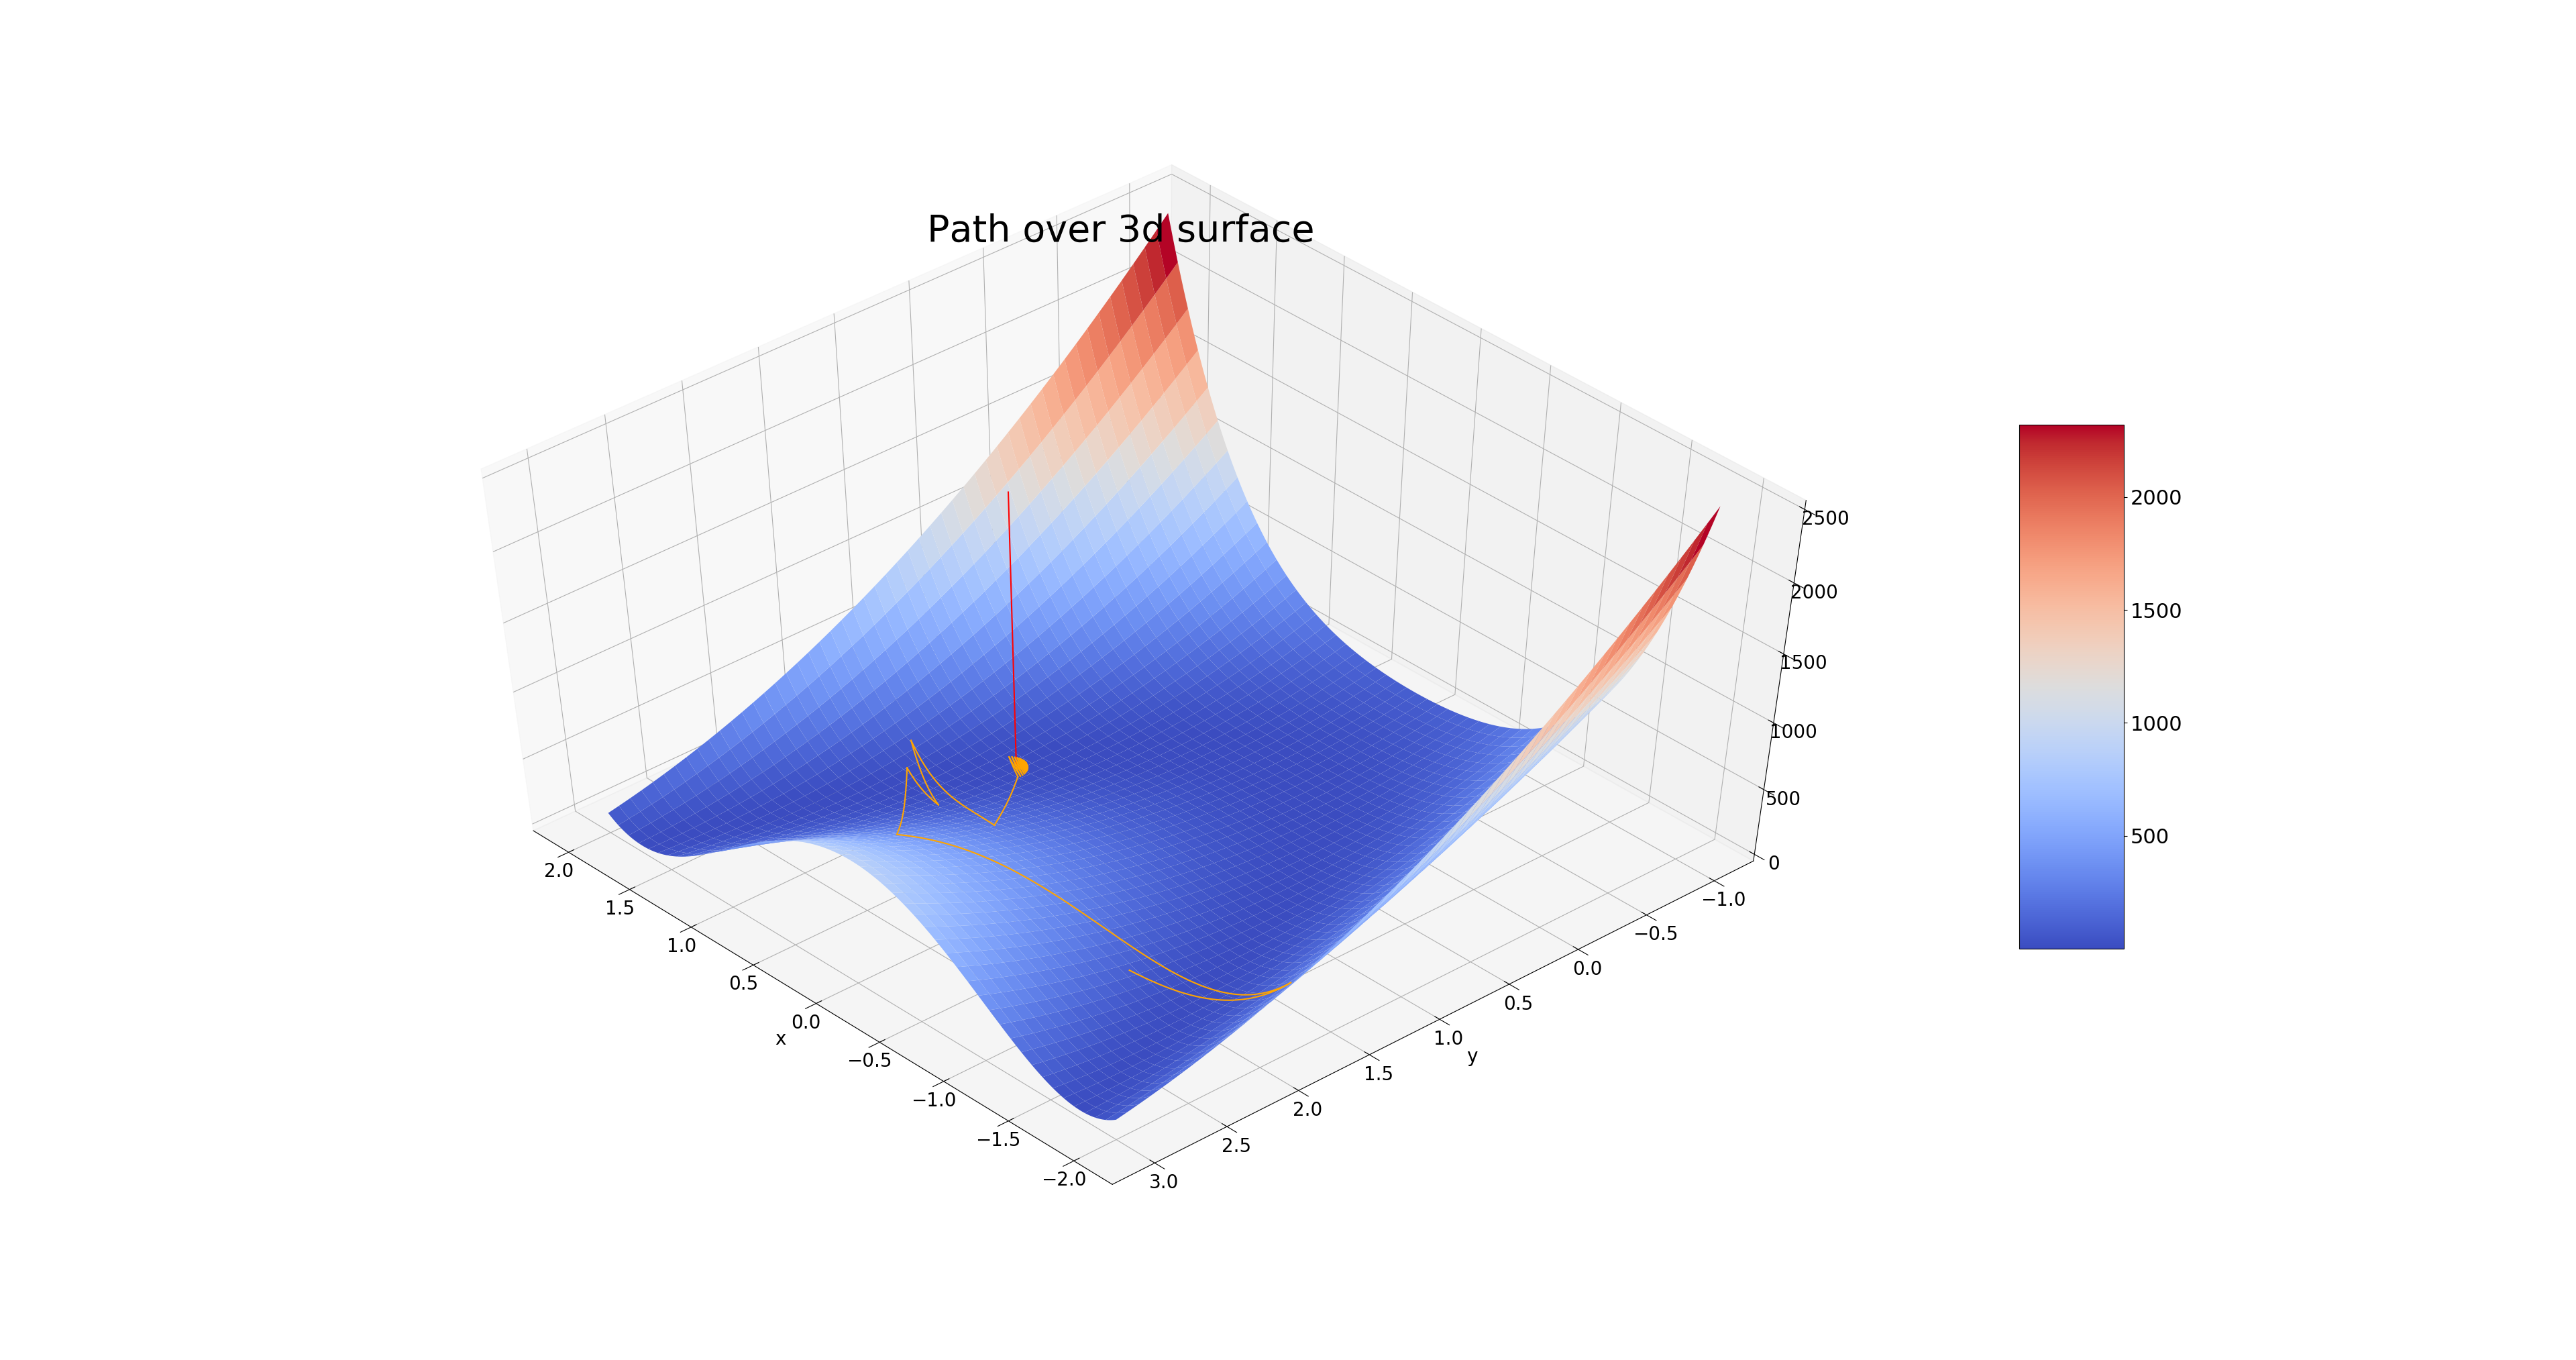
\includegraphics[width=1.5\textwidth]{Path_over_3d_surface.png}
\caption{Path over 3d surface. The orange indicates the path, the red the minimum (1,1). }
\end{figure}

A plot of how many times the walk converges you can see in the following figure. There we generated some random points and tracked how many of them converged in a certain amount of steps, given a certain $\eta$.
We chose the logarithm for $\eta$ so it can vary widely so we can find an optimal $\eta$.

\begin{figure}[H]
\hspace*{-6cm}
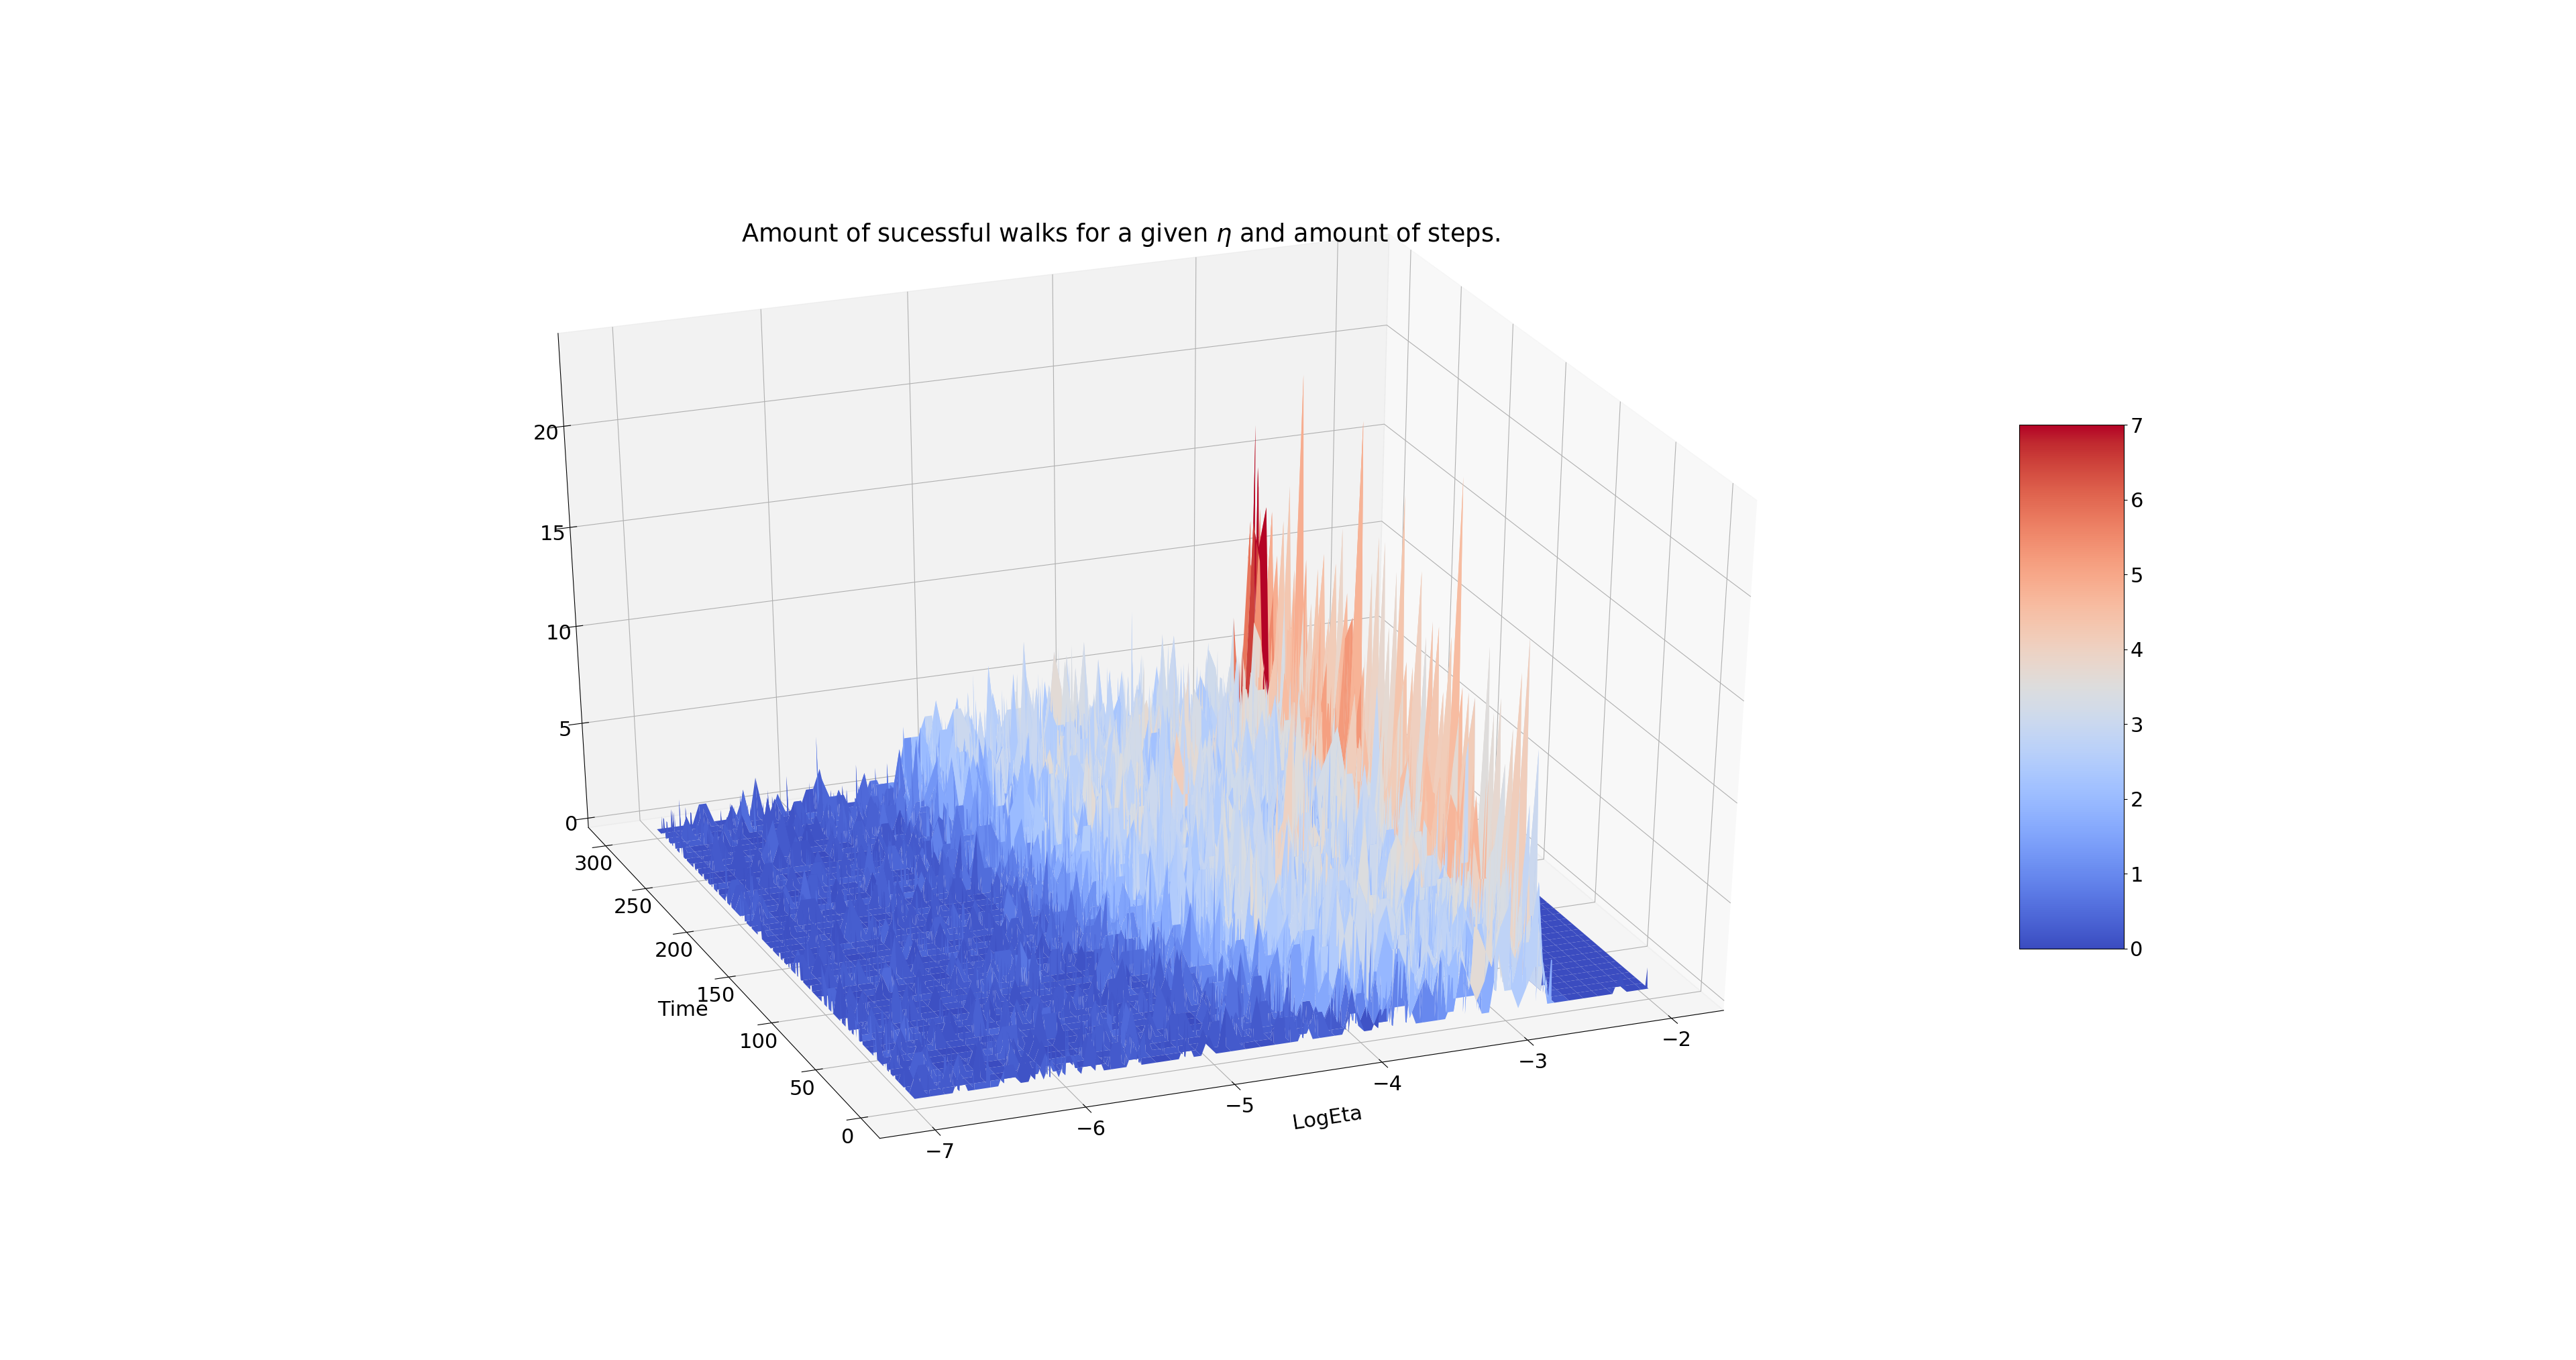
\includegraphics[width=1.5\textwidth]{3dError.png}
\caption{How many random paths converge given the amount of steps and the logarithm of $\eta$.}
\end{figure}

\end{enumerate}

	
\end{document}